\chapter{Implementation}

\section{Work Done}
The system built uses two retrieval techniques, suggestions based on topical and collaborative filtering. The users were given the liberty to select the first movie. Based on the above described methodology the co-view graph was used to calculate the score of all the other movies with respect to the current movie. The top ten movies were ranked and suggested to the user. \par
Our work incorporated both the user feedback and topic based on inverted index. This allowed our model to be robust. The user feedback also made room for unrelated movie recommendations. This was because the during the process of collecting co views users tend to deviate from the genres and teleport to some random genre. Hence those changes were visible in the co-view graph.

\section{Results and Analysis}

The following section describes the evaluation methodology, metrics used and the evaluation outcomes. We have used, user-centered evaluation metrics -- watch time, completion rate, abandonment rate.

\subsection{Evaluation Methodology}
There are many ways of evaluating systems like the one presented here (ToViS) -- online studies, user studies and historical data based user simulation. We must note that the sample test subjects chosen must represent the population subjects as much as possible. This is necessary to avoid any bias in decision and perception resulting from personal judgments. In addition to selecting the `perfect sample', explicit feedback collection from the selected users might result in intrusion and irritation.\par
If a user is to evaluate the given system would result in varied opinions based on a lot of `bias' factors -- culture, emotion, location etc. Table \ref{tab:2} represents the \textbf{Likert Evaluation} of the proposed system with respect to the experimental setup (section 3.1). The following section presents a much more apt evaluation methodology.

\begin{table}[h]
  \centering
  \bgroup
  \def\arraystretch{1.5}
  \caption{Summary of Likert Evaluation (20 users)}
  \label{tab:2}
  \begin{tabular}{>{\raggedright}p{4.5cm}>{\raggedright}p{1.8cm}>{\raggedright}p{1.8cm}>{\raggedright}p{1.8cm}>{\raggedright}p{1.9cm}>{\raggedright}p{1.9cm}} 
    \toprule
    \textbf{Question Asked} & \textbf{Strongly Agree} & \textbf{Agree} & \textbf{Neutral} & \textbf{Disagree} & \textbf{Strongly Disagree} \tabularnewline
    \midrule
     Did the recommender system recommend relevant videos? & 3 & 8 & 6 & 1
& 2 \tabularnewline
     Did your session time increase as result of suggestions? & 1 & 3 & 10 & 4 & 2 \tabularnewline
     Did you have Overall Satisfaction? & 4 & 6 & 7 & 2 & 1 \tabularnewline
    \bottomrule
  \end{tabular}
  \egroup
\end{table}

\subsection{Evaluation Metrics and Evaluation}

We have used much more apt evaluation metrics that were user centered. \textbf{Watch time} is the total time a user spends watching videos (movies) on ToViS. \textbf{Completion rate} is the number of videos that were presented to the user by ToViS and were watched completely. \textit{Abandonment rate} is the number of movies (videos) that the user watches up-until the point where the user \textit{does not} continue the session (watch any of the recommendations). \par
The evaluation of the system with the above mentioned metrics has been carried out in the experimental setup (section 3.1). Watch time (see Figure \ref{res:1}), Completion rate (see Figure \ref{res:2}) and Abandonment rate (see Figure \ref{res:3}) were captured for all 20 users and then these were averaged for overall evaluation (see Figure \ref{res:4}). Figures \ref{res:5} to \ref{res:8} represent the User Interface for ToViS. 

\begin{figure}
	\centering
	\label{res:1}
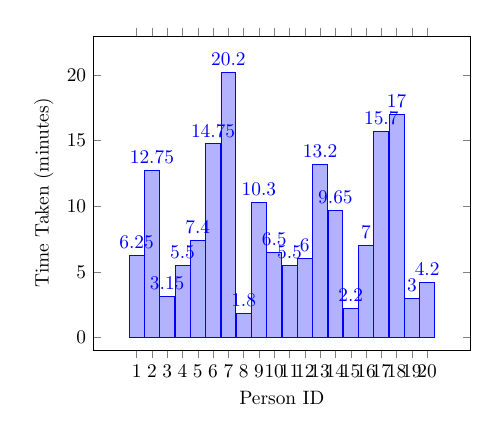
\begin{tikzpicture}[scale=0.7]
	\begin{axis}[
	    ybar,
        bar width=0.27cm,
    	enlargelimits=0.15,
    	legend style={at={(0.5,-0.15)},
      	anchor=north,legend columns=-1},
        xlabel={Person ID},
    	ylabel={Time Taken (minutes)},
    	symbolic x coords={1, 2, 3, 4, 5, 6, 7, 8, 9, 10, 11, 12, 13, 14, 15, 16, 17, 18, 19, 20},
    	xtick=data,
    	nodes near coords,
    	nodes near coords align={vertical},
    ]
	\addplot coordinates {(1, 6.25) (2, 12.75) (3, 3.15) (4, 5.50) (5, 7.40) (6, 14.75) (7, 20.20) (8, 1.80) (9, 10.30) (10, 6.5) (11, 5.5) (12, 6) (13, 13.20) (14, 9.65) (15, 2.2) (16, 7) (17, 15.70) (18, 17) (19, 3) (20, 4.2)};
    \end{axis}
\end{tikzpicture}
	\caption{Watch Time for 20 Users (Based on Experimental Setup)}
\end{figure}


\begin{figure}
	\centering
	\label{res:2}
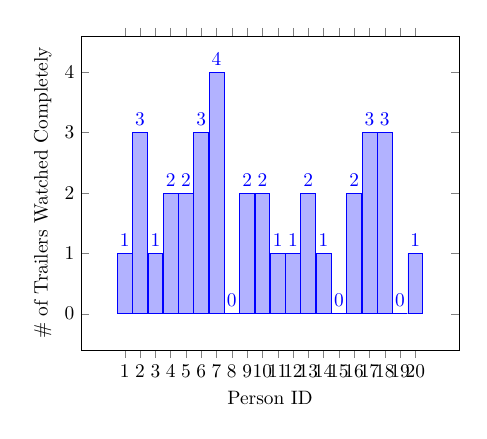
\begin{tikzpicture}[scale=0.7]
	\begin{axis}[
	    ybar,
        bar width=0.27cm,
    	enlargelimits=0.15,
    	legend style={at={(0.5,-0.15)},
      	anchor=north,legend columns=-1},
        xlabel={Person ID},
    	ylabel={\# of Trailers Watched Completely},
    	symbolic x coords={1, 2, 3, 4, 5, 6, 7, 8, 9, 10, 11, 12, 13, 14, 15, 16, 17, 18, 19, 20},
    	xtick=data,
    	nodes near coords,
    	nodes near coords align={vertical},
    ]
	\addplot coordinates {(1, 1) (2, 3) (3, 1) (4, 2) (5, 2) (6, 3) (7, 4) (8, 0) (9, 2) (10, 2) (11, 1) (12, 1) (13, 2) (14, 1) (15, 0) (16, 2) (17, 3) (18, 3) (19, 0) (20, 1)};
    \end{axis}
\end{tikzpicture}
	\caption{Completion Rate for 20 Users (Based on Experimental Setup)}
\end{figure}

\begin{figure}
	\centering
	\label{res:3}
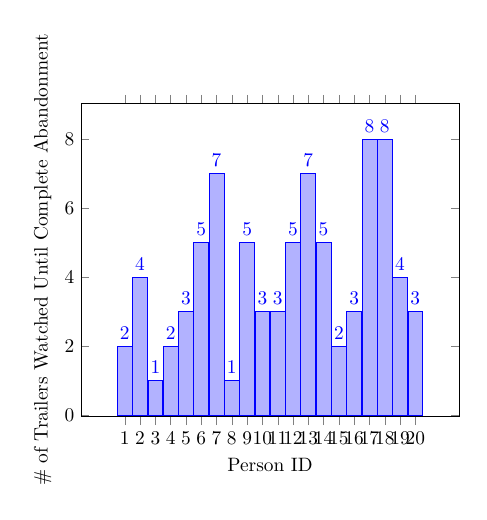
\begin{tikzpicture}[scale=0.7]
	\begin{axis}[
	    ybar,
        bar width=0.27cm,
    	enlargelimits=0.15,
    	legend style={at={(0.5,-0.15)},
      	anchor=north,legend columns=-1},
        xlabel={Person ID},
    	ylabel={\# of Trailers Watched Until Complete Abandonment},
    	symbolic x coords={1, 2, 3, 4, 5, 6, 7, 8, 9, 10, 11, 12, 13, 14, 15, 16, 17, 18, 19, 20},
    	xtick=data,
    	nodes near coords,
    	nodes near coords align={vertical},
    ]
	\addplot coordinates {(1, 2) (2, 4) (3, 1) (4, 2) (5, 3) (6, 5) (7, 7) (8, 1) (9, 5) (10, 3) (11, 3) (12, 5) (13, 7) (14, 5) (15, 2) (16, 3) (17, 8) (18, 8) (19, 4) (20, 3)};
    \end{axis}
\end{tikzpicture}
	\caption{Completion Rate for 20 Users (Based on Experimental Setup)}
\end{figure}

\begin{figure}
	\centering
	\label{res:4}
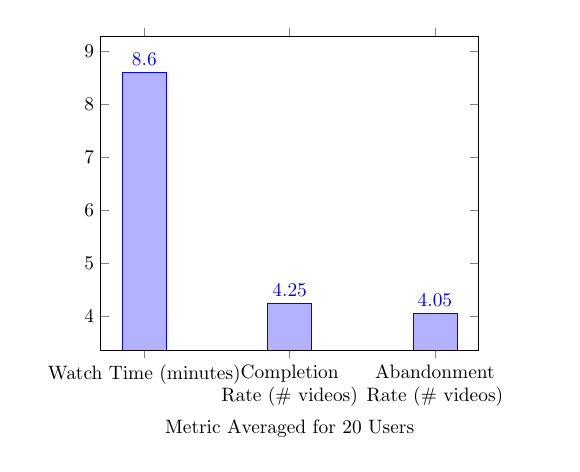
\begin{tikzpicture}[scale=0.7]
	\begin{axis}[
	    ybar,
        x tick label style={text width=4cm, align=center},
        bar width=0.8cm,
    	enlargelimits=0.15,
    	legend style={at={(0.5,-0.15)},
      	anchor=north,legend columns=-1},
        xlabel={Metric Averaged for 20 Users},
    	symbolic x coords={Watch Time (minutes), Completion Rate (\# videos), Abandonment Rate (\# videos)},
    	xtick=data,
    	nodes near coords,
    	nodes near coords align={vertical},
    ]
	\addplot coordinates {(Watch Time (minutes), 8.6025) (Completion Rate (\# videos), 4.25) (Abandonment Rate (\# videos), 4.05)};
    \end{axis}
\end{tikzpicture}
	\caption{Averaged Evaluation Metrics Used for User Relevance Evaluation}
\end{figure}

\begin{figure}[htb]
\centering
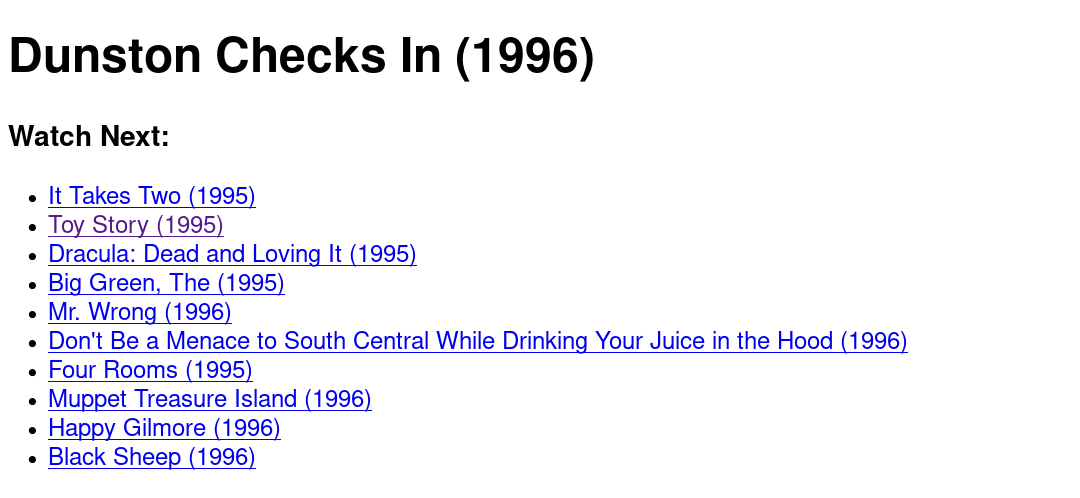
\includegraphics[scale=0.35]{images/img1}
\caption{User Interface for ToViS (I)}
\label{res:5}
\end{figure}

\begin{figure}[htb]
\centering
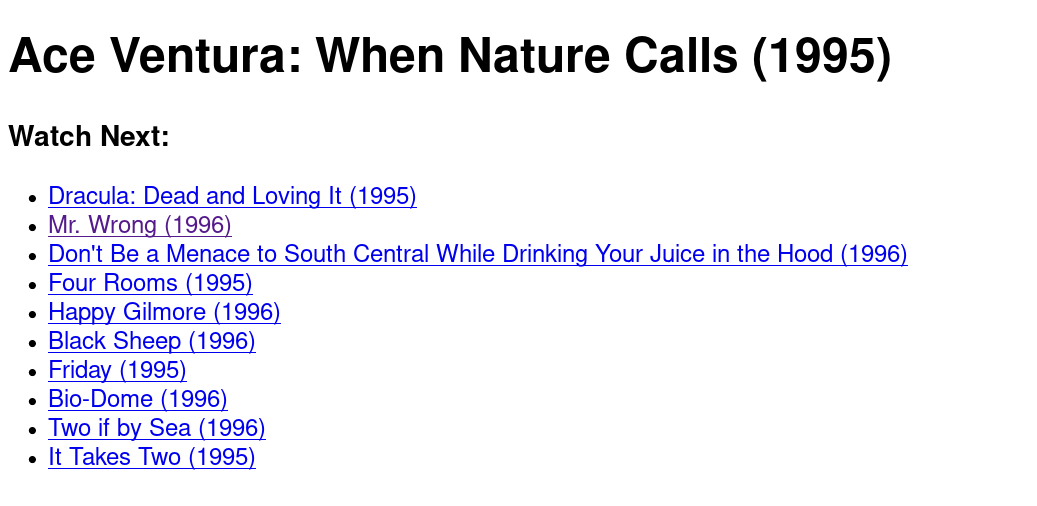
\includegraphics[scale=0.35]{images/img2}
\caption{User Interface for ToViS (II)}
\label{res:6}
\end{figure}

\begin{figure}[htb]
\centering
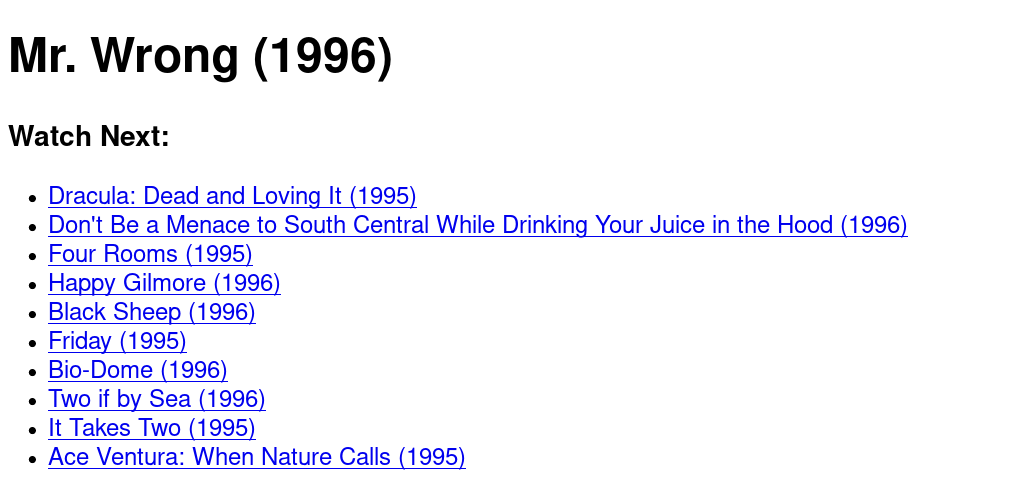
\includegraphics[scale=0.35]{images/img3}
\caption{User Interface for ToViS (III)}
\label{res:7}
\end{figure}

\begin{figure}[htb]
\centering
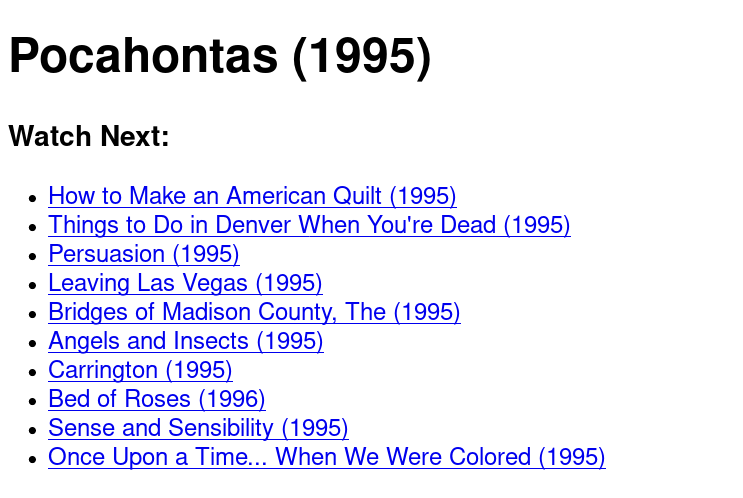
\includegraphics[scale=0.35]{images/img4}
\caption{User Interface for ToViS (IV)}
\label{res:8}
\end{figure}


\section{Innovative Work}

We added a novel concept of building the co-view graph by approaching a wide range of users and constructing a feedback loop. These metrics formed the basis for our model which was later coupled with the topic based recommendations.

\section{Details of each individual's work w.r.t. project tasks}

The individual contributions and the project time-line has been progressively represented in the form of a Gantt chart as in Figure \ref{contr:1}.

\begin{figure}[htb]
\centering
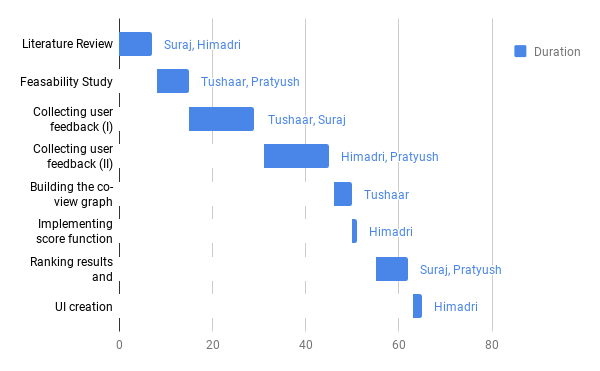
\includegraphics[scale=0.7]{images/chart}
\caption{Gantt Chart Representing the Work Flow and Individual Contributions}
\label{contr:1}
\end{figure}